\section{Comparación de Performance}

\subsection{Performance: Caso Exitoso - Paridad}
\begin{frame}
\begin{center}
\Large{Cuando todas las validaciones pasan...}
\end{center}

\begin{exampleblock}{Comando: ./gradlew demoCompare}
\begin{itemize}
\item \textbf{Reactive (CompletableFuture)}: ~520ms
\item \textbf{Structured Concurrency}: ~520ms
\item \textbf{Resultado}: Misma performance en casos exitosos
\end{itemize}
\end{exampleblock}


\begin{block}{¿Por qué iguales?}
Ambos ejecutan las 4 validaciones en paralelo y esperan que todas terminen:
\begin{itemize}
\item Balance: 500ms, Card: 300ms, Expiration: 200ms, PIN: 400ms
\item \textbf{Total}: max(500, 300, 200, 400) = 500ms + overhead $\approx$ 520ms
\end{itemize}
\end{block}
\end{frame}

\subsection{Performance: Caso Fallido - Ventaja Dramática}
\begin{frame}
\begin{center}
\Large{Cuando una validación falla...}
\end{center}

\begin{columns}
\column{0.5\textwidth}
\begin{alertblock}{Comando: demoCompareFailure}
\begin{itemize}
\item \textbf{Reactive}: ~570ms
\item \textbf{Structured}: ~230ms
\item \textbf{Mejora}: \textcolor{red}{\textbf{60\% más rápido}}
\end{itemize}
\end{alertblock}

\begin{block}{¿Por qué?}
\begin{itemize}
\item \textbf{Reactive}: allOf() espera TODAS
\item \textbf{Structured}: Cancela automático
\end{itemize}
\end{block}

\column{0.5\textwidth}
\begin{center}
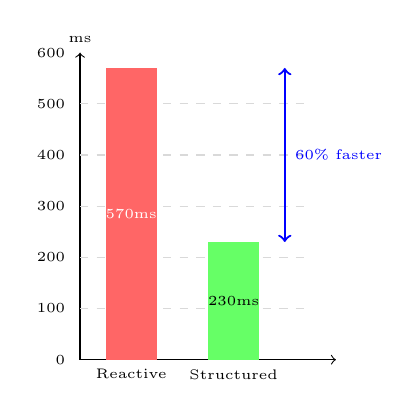
\begin{tikzpicture}[scale=0.65]
    % Y axis
    \draw[->] (0,0) -- (0,6) node[anchor=south] {\tiny ms};
    % X axis
    \draw[->] (0,0) -- (5,0);

    % Grid lines
    \foreach \y in {1,2,3,4,5}
        \draw[dashed, gray!30] (0,\y) -- (4.5,\y);

    % Y axis labels
    \node[anchor=east] at (-0.1,0) {\tiny 0};
    \node[anchor=east] at (-0.1,1) {\tiny 100};
    \node[anchor=east] at (-0.1,2) {\tiny 200};
    \node[anchor=east] at (-0.1,3) {\tiny 300};
    \node[anchor=east] at (-0.1,4) {\tiny 400};
    \node[anchor=east] at (-0.1,5) {\tiny 500};
    \node[anchor=east] at (-0.1,6) {\tiny 600};

    % Reactive bar (570ms ≈ 5.7 units)
    \fill[red!60] (0.5,0) rectangle (1.5,5.7);
    \node[anchor=north, font=\tiny] at (1,0) {Reactive};
    \node[font=\tiny, white] at (1,2.85) {570ms};

    % Structured bar (230ms ≈ 2.3 units)
    \fill[green!60] (2.5,0) rectangle (3.5,2.3);
    \node[anchor=north, font=\tiny] at (3,0) {Structured};
    \node[font=\tiny] at (3,1.15) {230ms};

    % Arrow showing difference
    \draw[<->, thick, blue] (4,2.3) -- (4,5.7) node[midway, right, font=\tiny] {60\% faster};

\end{tikzpicture}
\end{center}
\end{columns}

\begin{exampleblock}{Resultado}
Mejor UX y menor uso de recursos en errores
\end{exampleblock}
\end{frame}

% \begin{frame}
% \frametitle{Comparación Justa: awaitAll() vs allOf()}
% \begin{center}
% \textbf{Para ser justos... también creamos StructuredPaymentProcessor}
% \end{center}
% 
% 
% \begin{block}{StructuredTaskScope.open(awaitAll())}
% \begin{itemize}
% \item Usa \texttt{awaitAll()} en lugar del fail-fast por defecto
% \item Misma lógica que \texttt{CompletableFuture.allOf()}
% \item Performance idéntica en ambos casos (520ms éxito, 570ms fallo)
% \end{itemize}
% \end{block}
% 
% 
% \begin{exampleblock}{Aún así, Structured Concurrency gana}
% \begin{itemize}
% \item \textbf{Código más limpio}: Sin callbacks ni exception wrapping
% \item \textbf{Resource management}: Try-with-resources automático
% \item \textbf{Debugging}: Stack traces normales y claros
% \item \textbf{Opción by default}: Fail-fast sin configuración extra
% \end{itemize}
% \end{exampleblock}
% \end{frame}

